
\part{Analizador léxico}


\chapter{Análisis léxico: Especificación de los tokens}
    
    \section{Espacios}
    
        \subsection{Descripción}
        
            Usamos este tipo de Token para representar el conjunto de espacios, aunque este Token será ignorado desde el nivel sintáctico.
        
            A la hora de interpretar el documento, emplearemos 2 autómatas. Uno para interpretar los espacios convencionales, y otro para interpretar los saltos de linea, ya que a medida que vamos leyendo el documento iremos contando el número linea para reportarlo en caso de error.
        
        \subsection{Atributos}
        
            Ninguno
            
	    \subsection{Espacios normales}
     
            \subsubsection{Expresión regular}
                \begin{lstlisting}[language=Perl]
[\ \t]+
                \end{lstlisting}

            \subsubsection{Autómata}
            
                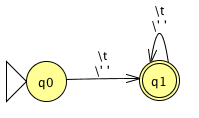
\includegraphics[scale=.7]{../Design/jflap/Espacio.png}
                
        \subsection{Saltos de linea}
        
            \subsubsection{Expresión regular}
            
                \begin{lstlisting}[language=Perl]
\n|\r|\r\n
                \end{lstlisting}
                
            \subsubsection{Autómata}
         
                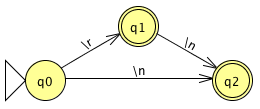
\includegraphics[scale=.7]{../Design/jflap/Salto_de_linea.png}
            
        \subsection{Notas}
        
            \begin{itemize}
            
                \item Con el método NextToken de la clase Tokenizer, podemos indicar si queremos filtrar los espacios y/o los saltos de linea.
            
            \end{itemize}
            
            \hfill
            \clearpage
            
            
            
    \section{Separadores}
    
        \subsection{Descripción}
        
            Usamos este tipo de Token para representar el conjunto de separadores :
            
            \begin{itemize}
                \item Paréntesis. Empleados para indicar los argumentos de los procedimientos.
                \item Punto y coma. Empleados para separar las instrucciones.
                \item Dos puntos. Para separar el tipo de los identificadores en las declaraciones de variables.
                \item Coma. Para separar los argumentos de los procedimientos, y los identificadores en las declaraciones de las variables.
            \end{itemize}
            
        \subsection{Expresión regular}
            
             \begin{lstlisting}[language=Perl]
[(),:;]
             \end{lstlisting}


        \subsection{Autómata}
            
	        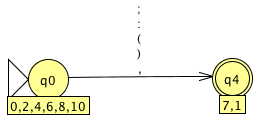
\includegraphics[scale=.7]{../Design/jflap/Separador.png}
	        
        \subsection{Atributos}
        
            \begin{itemize}
                \item Número de linea
                \item Número de columna
                \item Valor.
            \end{itemize}
            
            \hfill
            \clearpage
            
     
    
    \section{Comentario}
    
        \subsection{Descripción}
        
            Usamos este tipo de Token para representar los comentarios, aunque este Token será ignorado desde el nivel sintáctico.
            
            Los comentarios pueden ser multilinea, y aceptan cualquier contenido en su interior hasta encontrar el cierre del comentario.
        
        \subsection{Expresión regular}
            
             \begin{lstlisting}[language=Perl]
\/\*([^*]|(\*+[^*\/]))*\*+\/
             \end{lstlisting}
            
        \subsection{Autómata}
        
            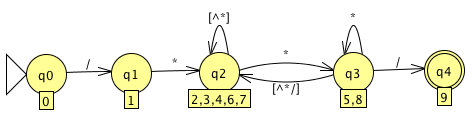
\includegraphics[scale=.7]{../Design/jflap/Comentario.png}

        \subsection{Atributos}
        
            \begin{itemize}
                \item Número de linea.
                \item Número de columna.
                \item Valor.
            \end{itemize}
            
            \hfill
            \clearpage
            


	\section{Identificador}

        \subsubsection{Descripción}
        
            Usamos este tipo de Token para representar un identificador.
            
            Los identificadores son de tipo Ada con subrayado: Empiezan por carácter alfabético, puede contener caracteres alfanuméricos o guión bajo, pero no puede comenzar ni terminar con un guión bajo ni puede contener dos guiones bajos seguidos.
            
        \subsection{Expresión regular}

            \begin{lstlisting}[language=Perl]
[a-zA-Z](_?[a-zA-Z0-9])*
            \end{lstlisting}

        \subsection{Autómata}
        
            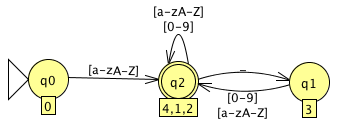
\includegraphics[scale=.7]{../Design/jflap/Identificador.png}

        \subsection{Atributos}
        
            \begin{itemize}
                \item Número de linea.
                \item Número de columna.
                \item Valor.
            \end{itemize}

            \hfill
            \clearpage
            



	\section{Constante entera}
    
        \subsection{Descripción}
        
            Usamos este tipo de Token para representar las constantes enteras.
        
        \subsection{Expresion regular}
        
            \begin{lstlisting}[language=Perl]
[0-9]+
            \end{lstlisting}

        \subsection{Autómata}
        
	        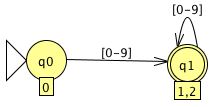
\includegraphics[scale=.7]{../Design/jflap/Constante_entera.png}

        \subsection{Atributos}
        
            \begin{itemize}
                \item Número de linea.
                \item Número de columna.
                \item Valor.
            \end{itemize}

            \hfill
            \clearpage
            
            
            
            
	\section{Constante real}

        \subsection{Descripción}

            Usamos este tipo de Token para representar las constantes reales, es decir números reales con decimales y exponencial.

        \subsection{Expresion regular}

            \begin{lstlisting}[language=Perl]
[0-9]+\.[0-9]+([eE][+\-]?[0-9]+)?
            \end{lstlisting}

        \subsection{Autómata}

            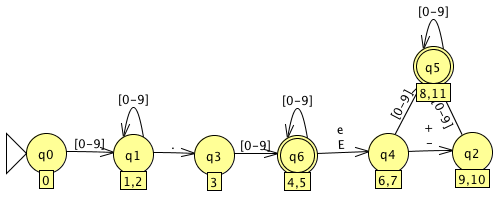
\includegraphics[scale=.7]{../Design/jflap/Constante_real.png}

        \subsection{Atributos}

            \begin{itemize}
                \item Número de linea.
                \item Número de columna.
                \item Valor.
            \end{itemize}

            \hfill
            \clearpage




	\section{Operadores}

        \subsection{Descripción}
        
            Usamos este tipo de Token para representar los operadores :
            
            \begin{itemize}
            
                \item Aritméticos
                \item Relacionales
                \item Operador asignación
                
            \end{itemize}
        
        \subsection{Operadores aritméticos}
        
            \begin{lstlisting}[language=Perl]
[+-*/]
            \end{lstlisting}

        \subsection{Operadores relacionales}

            \begin{lstlisting}[language=Perl]
[<>]|[/<>=]=
            \end{lstlisting}
            
        \subsection{Operador asignación}

            \begin{lstlisting}[language=Perl]
=
            \end{lstlisting}

        \subsection{Todos los operadores}

            \begin{lstlisting}[language=Perl]
[+-*/]|[<>]|[/<>=]=|=
            \end{lstlisting}

        \subsection{Autómata Operadores}

            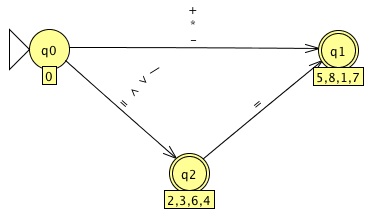
\includegraphics[scale=.7]{../Design/jflap/Operadores.png}

        \subsection{Atributos}

            \begin{itemize}
                \item Número de linea.
                \item Número de columna.
                \item Valor.
            \end{itemize}

            \hfill
            \clearpage



\section{Autómata competo unificado}

         \hspace{-7.8em}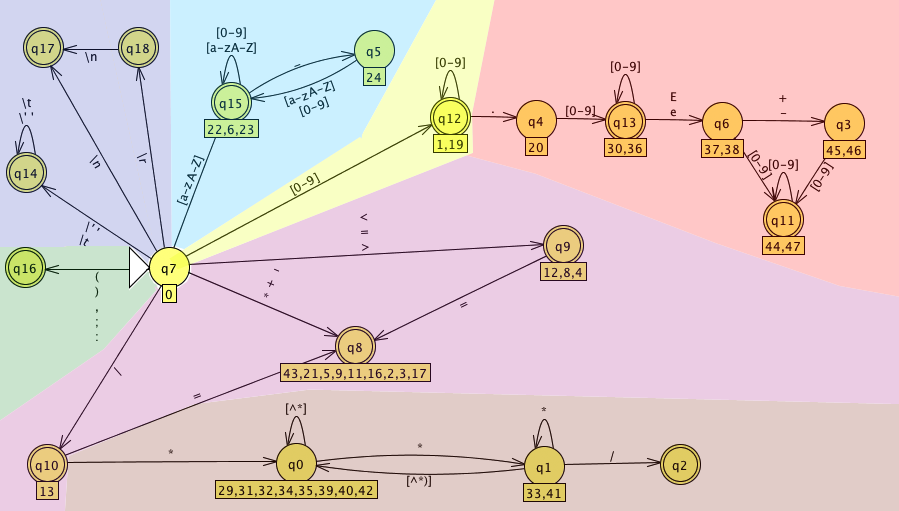
\includegraphics[scale=.61]{../Design/jflap/automata.png}

            \hfill
            \clearpage


 
\section{Listado de palabras reservadas}
    
        \subsection{Descripción}
        
        La palabras reservadas son identificadores reservados con un significado especial en nuestro lenguaje.
        
        \begin{itemize}
             \item programa
             \item procedimiento
             \item entrada
             \item salida
             \item si
             \item entonces
             \item fin
             \item hacer
             \item mientras
             \item salir
             \item get
             \item put\_line
       \end{itemize}

       \hfill
       \clearpage



